\subsection{Cinemática de la PGS}
\label{section: kinematics}

La PGS puede ser modelada en un inicio por medio de su 
cinemática inversa. Observando el modelo en la figura 
\ref{fig: gough stewart diagram} se puede formular lo 
siguiente:

 \begin{figure}[ht]
    \centering
    \import{./img/}{goughStewart.pdf_tex}
    \caption{Diagrama de la plataforma Gough Stewart.}
    \label{fig: gough stewart diagram}
\end{figure}

\begin{equation} \label{plat_grl}
p_i = d + Ra_i = b_i + l_i
\end{equation}

Siendo $Ra_i$ el lugar donde un extremo del actuador en la 
plataforma es colocado, el valor $b_i$ es el lugar donde el 
otro extremo del actuador es colocado en la base y $d$ es la 
distancia que debe de moverse la plataforma respecto de la 
base. Definimos $R$ como la matriz de rotación extrínseca de 
la plataforma respecto a la base. 

\begin{equation}
R = R_zR_yR_x = R_{xyz}
\end{equation}

El actuador es un pistón controlado por el largo y tomando 
en cuenta que el valor del actuador es $l_i$, podemos 
reescribir la ecuación \ref{plat_grl} de la siguiente 
manera.

\begin{equation}
l_i = d + Ra_i - b_i
\end{equation}

El vector $l_i$ se obtiene como coordenadas $[x\ y\ z]^T$ al 
cual se debe aplicar la norma para obtener la dimensión del 
actuador y será la coordenada generalizada del pistón 
i-ésimo de la plataforma.

\begin{equation}\label{eq_coordgral}
q_i = ||l_i|| = \sqrt{l_i^Tl_i}
\end{equation}

De la ecuación (\ref{eq_coordgral}) se obtendrá el jacobiano 
para después despejar el twist y utilizar los valores de 
velocidad lineal y angular de la plataforma para el 
desarrollo del control por fuerzas. Para obtener el 
jacobiano se plantea la siguiente ecuación

\begin{equation} \label{equgral_q}
J\dot{q}=\nu
\end{equation}

La ecuación \ref{eq_coordgral} al ser derivada respecto al 
tiempo es parecido a la ecuación del jacobiano en la 
solución de las velocidades de las coordenadas 
generalizadas.

\begin{equation}
\frac{d}{dt}q = \frac{d}{dt}||l_i|| = \frac{d}{dt}\sqrt{l_i^Tl_i} 
\end{equation}

La ecuación anterior se desarrolla para tener la forma del 
jacobiano inverso:

\begin{equation}
\dot{q}=J^{-1} \nu = A \begin{bmatrix}
v_p\\
\omega
\end{bmatrix} \Rightarrow A = J^{-1}
\end{equation}

Desarrollamos la derivada de $||l_||i$:
\begin{equation}
\dot{q} = \frac{1}{2||l_i||} \dot{l_i} \cdot l_i + l_i \cdot \dot{l_i} = \frac{1}{||l_i||} \dot{l_i} \cdot l_i \\ \bigskip
\end{equation}

\begin{equation}
\dot{q}=\frac{1}{||l_i||}(\dot{d} + [\omega \times] Ra_i)\cdot(d + Ra_i -b_i) 
\end{equation}
\begin{equation*}
= \frac{1}{||l_i||}(v_p - [(Ra_i)\times]\omega)(l_i)
\end{equation*}

\begin{equation}
\dot{q} = v_p \cdot l_i - [(Ra_i)\times]\omega \cdot l_i 
\end{equation}
\begin{equation*}
= v_p \cdot l_i + [(Ra_i)\times]l_i \cdot \omega
\end{equation*}

\begin{equation}
\dot{q} = \frac{1}{||l_i||} v_p \cdot l_i + [(Ra_i)\times]l_i \cdot \omega
\end{equation}

\begin{equation} \label{jac_inv}
\dot{q} = \frac{1}{||l_i||} [l_i^T , [(Ra_i)\times]l_i^T] \begin{bmatrix}
v_p\\
\omega
\end{bmatrix}
\end{equation}

Con el desarrollo se encuentra que la jacobiana inversa 
parte de la ecuación \ref{jac_inv} y se define como:

\begin{equation}\label{jac_A}
A = J^{-1} = \begin{bmatrix}
\vec{u_i}^T & [(Ra_i)\times]\vec{u_i}^T
\end{bmatrix}
\end{equation}

Al invertir la matriz $A$ de la ecuación \ref{jac_A} se 
obtiene la jacobiana de la PGS, con la cual se obtendrán las 
velocidades lineales y angulares de la PGS.

\begin{equation*}
J = \begin{bmatrix}
\vec{u_i}^T & [(Ra_i)\times]\vec{u_i}^T
\end{bmatrix}^{-1}
\end{equation*}

Utilizando la Jacobiana y desarrollando la ecuación 
\ref{equgral_q} se obtienen las velocidades lineales y 
angulares de la PGS.

\begin{equation*}
\begin{bmatrix}
\vec{u_i}^T & [(Ra_i)\times]\vec{u_i}^T
\end{bmatrix}^{-1} \dot{q} = \begin{bmatrix}
v_p\\
\omega
\end{bmatrix}
\end{equation*}

\subsection{Dinámica de la PGS}

La dinámica del robot será desarrollada
con la siguiente implementación. 
La posición y orientación de una
antena parabólica (especificaciones en anexos)
de 250 lb (113.4 kg) será controlada con la 
plataforma Gough Stewart. 
La figura \ref{fig: antenna} muestra una vista simplificada
de la implementación.

Para el desarrollo de la dinámica del robot, se conoce que 
soportará en la plataforma un disco parabólico con masa de 



\begin{figure}
 \centering
 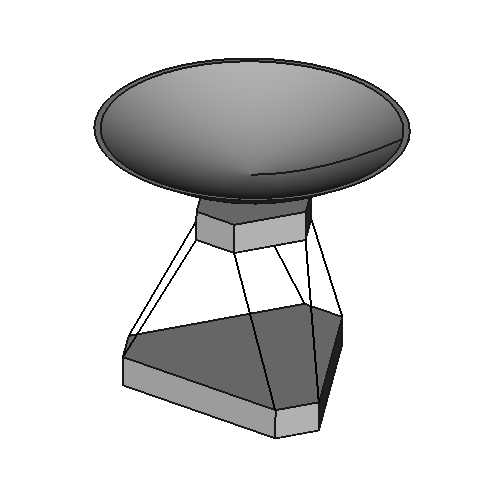
\includegraphics[scale=0.6]{img/implementation.png}
 % implementation.png: 495x490 px, 96dpi, 13.10x12.96 cm, bb=0 0 371 367
 \caption{Geometría simplificada de la implementación de la plataforma Gough Stewart.}
 \label{fig: antenna}
\end{figure}


Para obtener el modelo dinámico de la PGS con el 
disco se necesitan los valores de velocidad lineal y 
angular con respecto de la plataforma, se plantea la 
siguiente transformación.

\begin{equation} \label{equ_tr0-1}
\begin{split}
M_{6x6}\
\begin{bmatrix}
v_p^0\\
\omega^0
\end{bmatrix}  = \begin{bmatrix}
v_p^1\\
\omega^1
\end{bmatrix}
\end{split}
\end{equation}

En la ecuación \ref{equ_tr0-1} se identifica que al 
multiplicar las velocidades respecto a la base de la PGS se 
obtienen los valores de velocidades respecto a la 
plataforma. La matriz $M$ debe de tener la siguiente forma:

\begin{equation}
M = \begin{bmatrix}
I & 0_{3x3} \\
0_{3x3} & R^T
\end{bmatrix}
\end{equation}


Donde el primer bloque es la matriz identidad debido a que 
las velocidades lineales tanto de la base como de la 
plataforma son iguales, la matriz $E$ es la transformación 
de las velocidades angulares y tiene la siguiente forma:

\begin{equation*}
R^T = \begin{bmatrix}
R_{11} & R_{21} & R_{31}\\
R_{12} & R_{22} & R_{32}\\
R_{13} & R_{23} & R_{33}
\end{bmatrix}
\end{equation*}

Con la obtención del twist respecto a la plataforma del 
robot se pueden desarrollar las ecuaciones de energía. Se 
obtiene la energía potencial por medio de la altura del 
disco parabólico $dp$ sobre la plataforma del robot.

\begin{equation}
\begin{split}
P_{dp} = m_{dp}gh = [0\ 0\ m_{dp}g] \begin{bmatrix}
P_x\\
P_y\\
P_z\\
\end{bmatrix}\\
\\
P_z = d + R\begin{bmatrix}
0\\
0\\
cm_{dp}\\
\end{bmatrix}\\
\end{split}
\end{equation}

El punto $P_z$ es la altura del disco parabólico respecto a 
la base de la PGS. La energía cinética depende de las 
velocidades sobre el disco parabólico y se define

\begin{equation}
K = \frac{1}{2} \nu m_{dp} \nu = \frac{1}{2} \dot{q}^T J^T\ m\ J \dot{q}
\end{equation}
